\documentclass[a4paper,twoside]{ctexart}
\usepackage{geometry}
\geometry{margin=1cm,vmargin={0pt,1cm}}
\setlength{\topmargin}{-2cm}
\setlength{\paperheight}{23cm}
\setlength{\paperwidth}{18cm}
\setlength{\textheight}{19.6cm}
\setlength{\textwidth}{15cm}
\usepackage{makecell}
\usepackage{fancyhdr}
\usepackage{siunitx}
\usepackage{amssymb}
\usepackage{indentfirst}
\setlength{\parindent}{0.5em}

\pagenumbering{arabic}

% useful packages.
\usepackage{multirow}
\usepackage{caption}
\usepackage{mathrsfs}
\usepackage{amsfonts}
\usepackage{amsmath}
\usepackage{amsthm}
\usepackage{enumerate}
\usepackage{xcolor,graphicx,float,subfigure}
\usepackage{epstopdf}
\usepackage{multicol}
\usepackage{fancyhdr}
\usepackage{layout}
\usepackage{listings}
\usepackage{diagbox}
\lstset{language=Matlab}
\lstset{breaklines}
\lstset{extendedchars=false}
\usepackage[colorlinks,linkcolor=blue]{hyperref}
\usepackage{xcolor}
\usepackage{cite}
\usepackage[numbers,sort&compress]{natbib}
\setcitestyle{open={},close={}}
%\usepackage{natbibspacing}
%\renewcommand{\refname}{}
\usepackage{anyfontsize}

% English theorem environment
\theoremstyle{definition}
\newtheorem{proposition}[section]{Proposition}
\newtheorem{corollary}[section]{Corollary}
\newtheorem{definition}{Definition}[section]
\newtheorem{remark}[section]{Remark}
\newtheorem{example}[definition]{Example}
\newtheorem{exercise}[definition]{Exercise}
\newtheorem{theorem}[definition]{Theorem}
\newtheorem{lemma}[definition]{Lemma}
\newenvironment{solution}{\begin{proof}[Solution]}{\end{proof}}
\renewcommand{\proofname}{\noindent Proof}
% some common command
\newcommand{\dif}{\mathrm{d}}
\newcommand{\avg}[1]{\left\langle #1 \right\rangle}
\newcommand{\pdfrac}[2]{\frac{\partial #1}{\partial #2}}
\newcommand{\op}{\odot}
\newcommand{\Eabs}{E_{\mathrm{abs}}}
\newcommand{\Erel}{E_{\mathrm{rel}}}
\newcommand{\Ediv}{\mathrm{div}}%\div是除号
\newcommand{\lrq}[1]{\left( #1 \right)}
\newcommand{\avint}[1]{\frac{1}{\left|#1\right|}\int_{#1}}

\newcommand{\upcite}[1]{\textsuperscript{\textsuperscript{\cite{#1}}}} 

\makeatletter
\newcommand\sixteen{\@setfontsize\sixteen{17pt}{6}}
\renewcommand{\maketitle}{\bgroup\setlength{\parindent}{0pt}
\begin{flushleft}
\sixteen\bfseries \@title
\medskip
\end{flushleft}
\textit{\@author}
\egroup}
\renewcommand{\maketag@@@}[1]{\hbox{\m@th\normalsize\normalfont#1}}
\makeatother

%\CTEXsetup[format={\Large\bfseries}]{section}

\title{Maximum Principle Analysis}


\begin{document}
\maketitle

\section{}
\subsection{$\theta$-method}
\begin{definition}
  The $\theta$-method solves the heat equation (11.3) by 
  \begin{eqnarray}
  \label{eq:thetamethod}
  \begin{aligned}
  &\frac{U_i^{n+1} - U_i^{n}}{k} = \theta f(U_i^{n+1},t_{n+1}) + (1 - \theta) f(U_i^{n},t_{n})\\
  &=\frac{\nu}{h^2}[\theta(U_{i-1}^{n+1}-2U_{i}^{n+1}+U_{i+1}^{n+1})+(1-\theta)(U_{i-1}^{n}-2U_{i}^{n}+U_{i+1}^{n})],
  \end{aligned}
  \end{eqnarray}
  or, equivalently
  \begin{eqnarray}
  \label{eq:thetaform}
  \begin{aligned}
  &-2\theta r U_{i-1}^{n+1} + (1 + 4\theta r)U_{i}^{n+1} - 2\theta r U_{i+1}^{n+1}\\
  =&2(1-\theta)rU_{i-1}^{n}+[1-4(1-\theta)r]U_{i}^{n}+2(1-\theta)rU_{i+1}^{n},
  \end{aligned}
  \end{eqnarray}
  where $r = \frac{k\nu}{2h^2}$. Here $0 \le \theta \le 1$.
  \end{definition}
\begin{example}
	Set $\theta = 0$ in $\theta$-method, we get FTCS method and set $\theta = \frac{1}{2}$ we get Crank-Nicolson method.	
\end{example}
\begin{lemma}
	\label{le:thetaLTE}
	The LTE of the $\theta$-method is 
	\begin{eqnarray}
	\label{eq:LTE}
	\begin{aligned}
	\tau_i^{n+\frac{1}{2}} = O(k+h^2),
	\end{aligned}
	\end{eqnarray}
	i.e., this method is second order accurate in space and first order accurate in time.
\end{lemma}
\begin{proof}
	 To take maximum advantage of cancellations in the Taylor expansions, expand each term about the
	 point $(x_i , t_{n+\frac{1}{2}})$. We obtain
	 \begin{eqnarray}
	 \label{eq:LTEres}
	 \begin{aligned}
	 \tau_i^{n+\frac{1}{2}} &:= \frac{u(x_i,t_n+k) - u(x_i,t_n)}{k} \\
	 &\quad \ -\frac{\nu}{h^2}\theta(u(x_i-h,t_n+k)-2u(x_i,t_n+k)+u(x_i+h,t_n+k))\\
	 &\quad \ -\frac{\nu}{h^2}(1-\theta)(u(x_i-h,t_n)-2u(x_i,t_n)+u(x_i+h,t_n))\\
	 &=\left[u_t - u_{xx}\right] + \left[\left(\frac{1}{2}-\theta\right)ku_{xxt}-\frac{1}{12}h^2u_{xxxx}\right]\\
	 &\quad \
	 +\left[\frac{1}{24}k^2u_{ttt}-\frac{1}{8}k^2u_{xxtt}\right]+\left[\frac{1}{12}\left(\frac{1}{2}-\theta\right)kh^2u_{xxxxt}-\frac{2}{6!}h^4u_{xxxxxx}\right]+\cdots,
	 \end{aligned}
	 \end{eqnarray}
	 Notice the first term always cancels, hence we complete the proof.
\end{proof}
\begin{example}
	Set $\theta = \frac{1}{2}$, we see that the Crank–Nicolson method is always second order accurate
	in both space and time.
\end{example}
\begin{example}
	Set $\theta = \frac{1}{2} - \frac{h^2}{12k}$, we get a method whose LTE is $O(k^2+h^4)$. Note that this requires $h^2 \le 6k$ to ensure $\theta \ge 0$. In fact, this method is also absolutely stable. You can get it by verifying following \eqref{eq:cond0} is satisfied.
\end{example}
\begin{lemma}
	\label{le:stableoftheta}
	For the $\theta$-method \eqref{eq:thetamethod} to be absolutely stable, the following conditions must be satisfied:
	\begin{eqnarray}
	\label{eq:cond0}
	\begin{aligned}
	\begin{cases}
	r \le \frac{1}{4(1-2\theta)} , \quad 0 \le \theta < \frac{1}{2}, \\
	r > 0, \quad \frac{1}{2} \le \theta \le 1, 
	\end{cases}
	\end{aligned}
	\end{eqnarray}
	which imply the time-step limit $k \le \frac{h^2}{2(1-\theta)\nu}$ when $0 \le \theta < \frac{1}{2}$, and unconditionally stability when $\frac{1}{2} \le \theta \le 1$.
\end{lemma}

\begin{exercise}
	Prove Lemma \ref{le:stableoftheta}.
\end{exercise}

\begin{proof}
	We prove Lemma \ref{le:stableoftheta} by Von Neumann analysis. Set
	\begin{eqnarray}
	\begin{aligned}
	U_j^n = [g(\xi)]^n e^{ix_j\xi},
	\end{aligned}
	\end{eqnarray}
	then $U_j^{n+1} = g(\xi)U_j^n$ and \eqref{eq:thetamethod} give
	\begin{eqnarray}
	\begin{aligned}
	g(\xi) - 1 &= 2r[\theta g(\xi) + (1 - \theta)](e^{-i\xi h} - 2 + e^{i\xi h})\\
	&=2r[\theta g(\xi) + (1 - \theta)]\left(-4\sin^2{\left(\frac{\xi h}{2}\right)}\right)
	\end{aligned}
	\end{eqnarray}
	i.e.,
	\begin{eqnarray}
	\begin{aligned}
	g(\xi) = \frac{1-8(1-\theta)r\sin^2{\left(\frac{\xi h}{2}\right)}}{1+8\theta r \sin^2{\left(\frac{\xi h}{2}\right)}}.
	\end{aligned}
	\end{eqnarray}
	Because $r > 0$, and we are assuming that $0 \le \theta \le 1$, it is clear that we
	can never have $g(\xi) > 1$. Thus instability arises only through the possibility
	that $g(\xi) < −1$, which implies
	\begin{eqnarray}
	\begin{aligned}
	1-8(1-\theta)r\sin^2{\left(\frac{\xi h}{2}\right)} < -\left[1+8\theta r \sin^2{\left(\frac{\xi h}{2}\right)}\right]
	\end{aligned}
	\end{eqnarray}
	i.e.,
	\begin{eqnarray}
	\begin{aligned}
	8r(1-2\theta)\sin^2{\left(\frac{\xi h}{2}\right)} > 2.
	\end{aligned}
	\end{eqnarray}
	The mode most liable to instability is the one for which the left side is largest: $\xi h = \pi$. This is an unstable mode if
		\begin{eqnarray}
		\label{eq:cond1}
	\begin{aligned}
	r(1-2\theta) > \frac{1}{4}.
	\end{aligned}
	\end{eqnarray}
	Notice that if $\theta \ge \frac{1}{2}$, \eqref{eq:cond1} will never hold.
\end{proof}
\begin{theorem}
	The $\theta$-method is convergent.
\end{theorem}
\begin{proof}
	The proof is similar to the convergence of Crank–Nicolson method By noticing
	\begin{eqnarray}
	\label{eq:thetaB}
	\begin{aligned}
	B = (I-\theta kA)^{-1}[I+(1-\theta)kA]
	\end{aligned}
	\end{eqnarray}
	and
	\begin{eqnarray}
	\begin{aligned}
	\rho(B) = \max\left|\frac{1+(1-\theta)k\lambda_p}{1-\theta k\lambda_p}\right| \le 1.
	\end{aligned}
	\end{eqnarray}
	Then the proof is completed by Theorem 11.23 and Lemma \ref{le:thetaLTE}.
\end{proof}
\subsection{Discrete maximum principle}
\begin{theorem}[Maximum principle of the heat equation]
	If $u(x,t)$ is continuous on rectangle $\bar{\Omega} = [0,1]\times[0,T]$, and satisfies the heat equation (11.3) in $\Omega = (0,1) \times (0,T)$, then the maximum and minimum value of $u(x,t)$ over the rectangle is assumed either initially
	$(t = 0)$, or on the lateral sides $(x = 0, \text{or}\ x = 1)$.
\end{theorem}
\begin{example}
	If we denote the set of points comprising the three sides by $\Gamma = \{(x, t) \in \bar{\Omega}\ |\ t = 0 \ \text{or}\ x = 0\ \text{or}\ x = 1\}$, then the maximum principle can be written as
	\begin{eqnarray}
	\begin{aligned}
	\max_{(x,t) \in \bar{\Omega}}\{u(x,t)\} = \max_{(x,t) \in \Gamma}\{u(x,t)\},\\
	\min_{(x,t) \in \bar{\Omega}}\{u(x,t)\} = \min_{(x,t) \in \Gamma}\{u(x,t)\}.
	\end{aligned}
	\end{eqnarray}
\end{example}
\begin{theorem}[Discrete maximum principle]
	The $\theta$-method of \eqref{eq:thetamethod} with $0 \le \theta \le 1$ and $r \le \frac{1}{4(1 − \theta)} $ yields $U_j^n$ satisfying
		\begin{eqnarray}
	\label{eq:dismaxprcp}
	\begin{aligned}
	U_{min} \le U_j^n \le U_{max},
	\end{aligned}
	\end{eqnarray}
	where 
		\begin{eqnarray}
	\label{eq:Umin}
	\begin{aligned}
	U_{min} := \min{\{U_0^s,\ 0 \le s \le n;\ U_j^0,\ 0 \le j \le m+1; \ U_{m+1}^s,\ 0 \le s \le n\}},
	\end{aligned}
	\end{eqnarray}
	and
		\begin{eqnarray}
	\label{eq:Umax}
	\begin{aligned}
	U_{max} := \max{\{U_0^s,\ 0 \le s \le n;\ U_j^0,\ 0 \le j \le m+1; \ U_{m+1}^s,\ 0 \le s \le n\}}.
	\end{aligned}
	\end{eqnarray}
\end{theorem}
\begin{proof}
	We write \eqref{eq:thetaform} in the form
	\begin{eqnarray}
	\label{eq:thetanewform}
	\begin{aligned}
	 (1 + 4\theta r)U_{j}^{n+1} 
	=&\ 2\theta r (U_{j-1}^{n+1}+U_{j+1}^{n+1})+2(1-\theta)r(U_{j-1}^{n}+U_{j+1}^{n})\\
	&+[1-4(1-\theta)r]U_{j}^{n},
	\end{aligned}
	\end{eqnarray}
	Then under the hypotheses of the theorem all the coefficients on the right
	are nonnegative and sum to $(1 + 4\theta r)$. Now suppose that $U$ attains its maximum at an internal point, and this maximum is $U_j^{n+1}$, and let $U^*$ be the greatest of the five values of $U$ appearing on the right-hand side of \eqref{eq:thetanewform}. Then since the coefficients are nonnegative,
	\begin{eqnarray}
	\begin{aligned}
	(1 + 4\theta r)U_{j}^{n+1} 
	\le&\ 2\theta r (U^*+U^*)+2(1-\theta)r(U^*+U^*)\\
	&+[1-4(1-\theta)r]U^* = (1 + 4\theta r)U^*, 
	\end{aligned}
	\end{eqnarray}
	i.e., $U_{j}^{n+1} \le U^*$. But since
	$U_{j}^{n+1}$ is assumed to be the maximum value, we also have $U_{j}^{n+1} \ge U^*$, so $U_{j}^{n+1} = U^*$.  Indeed, the maximum value must also be attained at each
	neighbouring point which has a non-zero coefficient in \eqref{eq:thetanewform}. The same
	argument can then be applied at each of these points, showing that the
	maximum is attained at a sequence of points, until a boundary point
	is reached. The maximum is therefore attained at a boundary point.
	An identical argument shows that the minimum is also attained at a
	boundary point, and the proof is complete.
\end{proof}
\begin{theorem}
	Asuume the condition $r \le \frac{1}{4(1 − \theta)} $ holds, then the $\theta$-method \eqref{eq:thetamethod} is convergent with consistent initial and
	Dirichlet boundary data.
\end{theorem}
\begin{proof}
	Firstly we assume that numerical errors arise from the truncation
	errors of the finite difference approximations, but that the boundary
	values are used exactly. This part is the same as sufficiency of theorem 11.23.\\
	Apply the $\theta$-method \eqref{eq:thetaform} to the exact solution $u(x_i,t_n)$ and we obtain
	\begin{eqnarray}
	\label{eq:exactformula}
	\begin{aligned}
	 (1 + 4\theta r)u(x_{i},t_{n+1}) 
	=&\ 2\theta r (u(x_{i-1},t_{n+1})+u(x_{i+1},t_{n+1}))+2(1-\theta)r(u(x_{i-1},t_{n})+u(x_{i+1},t_{n}))\\
	&+[1-4(1-\theta)r]u(x_{i},t_{n}) + k \tau_i^{n+\frac{1}{2}},
	\end{aligned}
	\end{eqnarray}
	Subtracting \eqref{eq:exactformula} from \eqref{eq:thetanewform}, the global error $E_i^n = U_i^n - u(x_i,t_n)$ is determined from the relations
	\begin{eqnarray}
	\label{eq:errrelations}
	\begin{aligned}
	(1 + 4\theta r)E_{i}^{n+1} 
	=&\ 2\theta r (E_{i-1}^{n+1}+E_{i+1}^{n+1})+2(1-\theta)r(E_{i-1}^{n}+E_{i+1}^{n})\\
	&+[1-4(1-\theta)r]E_{i}^{n}- k \tau_i^{n+\frac{1}{2}}
	\end{aligned}
	\end{eqnarray}
	for $i = 1,2,\cdots,m$ and $n = 0,1,\cdots$ together with initial and boundary conditions. By assumption, $E_i^0$, $E_0^n$ and $E_{m+1}^n$ are all zero with $i = 0,1,\cdots,m+1$ and $n = 0,1,\cdots$ . Then we define 
	\begin{eqnarray}
	\begin{aligned}
	E^n := \max_{0 \le i \le m+1}\left|E_i^n\right| ,\quad \tau^{n+\frac{1}{2}} := \max_{1 \le i \le m}\left|\tau_i^{n+\frac{1}{2}}\right|.
	\end{aligned}
	\end{eqnarray}
	Because of the nonnegative coefficients, it follows that
	\begin{eqnarray}
	\begin{aligned}
	(1 + 4\theta r)E^{n+1} 
	\le\ 4\theta r E^{n+1} +E^{n} + k \tau^{n+\frac{1}{2}}
	\end{aligned}
	\end{eqnarray}
	and hence that
	\begin{eqnarray}
	\begin{aligned}
	E^{n+1} 
	\le\ E^{n} + k \tau^{n+\frac{1}{2}}.
	\end{aligned}
	\end{eqnarray}
	Since $E^0 = 0$, 
	\begin{eqnarray}
	\label{eq:errbound}
	\begin{aligned}
	E^{n} 
	\le k \sum_{0}^{n-1}\tau^{s+\frac{1}{2}} \le nk \max_{s} \tau^{s+\frac{1}{2}},
	\end{aligned}
	\end{eqnarray}
	and this tends to zero following from Lemma \ref{le:thetaLTE}. Suppose now that there are errors in the initial and boundary values of $U_i^n$ and denote them by $\epsilon_i^0$, $\epsilon_0^n$ and $\epsilon_{m+1}^n$ with $i = 0,1,\cdots m+1$ and $n = 0,1,\cdots$. Then the errors $E_i^n$  satisfy the
	recurrence relation \eqref{eq:errrelations} with initial and boundary values
	\begin{eqnarray}
	\begin{aligned}
	&E_i^0 = \epsilon_i^0, \quad i = 0,1,\cdots m+1,\\
	E_0^n &= \epsilon_0^n, \ E_{m+1}^n = \epsilon_{m+1}^n, \quad n = 0,1,\cdots.
	\end{aligned}
	\end{eqnarray}
	By Duhamel's principle, $E_i^n$ can be written as the sum of two
	terms. The first term satisfies \eqref{eq:errrelations} with zero initial and boundary
	values; this term is bounded by \eqref{eq:errbound}. The second term satisfies the
	homogeneous form of \eqref{eq:errrelations}, with the term of $\tau$ omitted, and with the given non-zero initial and boundary values. By the discrete maximum principle
	this term must lie between the maximum and minimum values of these
	initial and boundary values. Thus the error of the numerical solution
	will tend to zero, as required, provided that
	the initial and boundary values are consistent; that is, the errors in the
	initial and boundary values also tend to zero as $k,h$ tend to zero.
\end{proof}
\begin{example}
	The condition for discrete maximum principle, $r(1 − \theta) \le \frac{1}{4}$ , is very much more
	restrictive than that needed in stability, $r(1 −
	2\theta) \le \frac{1}{4}$. For example, the Crank–Nicolson method always satisfies the
	stability condition, but only if $r ≤\le \frac{1}{2}$ does it satisfy the condition given for a discrete maximum principle.\\
	Consider the model problem
	solved by the Crank–Nicolson method. The boundary conditions specify
	that the solution is zero at each end of the range, and the initial condition gives the values of $U_i^0$ to be zero except at the mid-point; the value at
	the mid-point is unity. This corresponds to a function with a sharp spike
	at $x = \frac{1}{2}$.
	\begin{figure}[!htp]                                                                       
		\centering                                                                                                                  
		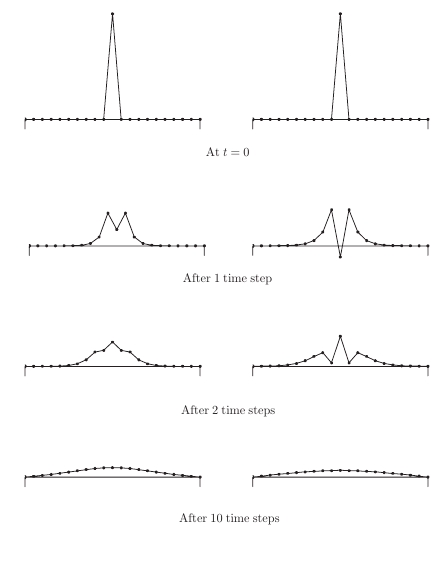
\includegraphics[width=7.4cm]{F3.png}                                           
		\caption*{The Crank–Nicolson method applied to the heat
			equation where the initial distribution has a sharp spike at the mid-point; $m = 19, h = 0.05$; left: $r = \frac{1}{2}$, right: $r = 1$.}                        
	\end{figure}
	
	\noindent In the case $r = 1$ , at the first time level the numerical solution becomes negative
	at the mid-point. This would normally be regarded as unacceptable. When $r = \frac{1}{2}$, the numerical values all lie between 0 and 1 as required. However, at the first time level the numerical solution shows two peaks, one each side of the mid-point. But the
	exact solution of the problem will have only a single maximum for all $t$.\\
	%These results correspond to a rather extreme case, and
	 The unacceptable behaviour only persists for a few time steps; thereafter the solution
	becomes very smooth in each case. However, they show that in a situation where we require to model some sort of rapid variation in the solution we shall need to use a value of $r$ somewhat smaller than the stability limit.
\end{example}
\end{document}

